% A short research note on directional recovery and real external comparisons.
\documentclass[UTF8,a4paper,fontset=windows]{ctexart}
\usepackage[margin=21mm,top=19mm,bottom=20mm]{geometry}
\usepackage{amsmath,amssymb,booktabs,tabularx,array,xcolor,graphicx,fancyhdr}
\definecolor{ink}{HTML}{193848}
\definecolor{accent}{HTML}{0C675C}
\definecolor{muted}{HTML}{46606B}
\setlength{\parindent}{0pt}
\setlength{\parskip}{.46em}
\setlength{\emergencystretch}{1.2em}
\graphicspath{{../imu-uwb-inekf/experiments/split_handoff/figures/}{imu-uwb-inekf/experiments/split_handoff/figures/}}
\renewcommand{\arraystretch}{1.18}
\pagestyle{fancy}\fancyhf{}\fancyhead[L]{\small\color{muted} IMU–UWB 定位 \quad / \quad 分量交接}
\fancyhead[R]{\small\color{muted} 数学模型与真实回放}
\fancyfoot[R]{\small\color{muted}\thepage}
\setlength{\headheight}{16pt}
\renewcommand{\headrulewidth}{.35pt}
\newcommand{\titleblock}[2]{{\color{accent}\small\bfseries #1}\par\vspace{.25em}{\color{ink}\LARGE\bfseries #2}\par\vspace{.25em}}
\newcommand{\topic}[1]{\par\vspace{.25em}{\color{accent}\bfseries #1}\par}
\newcommand{\unit}[1]{\,\mathrm{#1}}
\newcommand{\rank}{\operatorname{rank}}
\newcommand{\proj}{\operatorname{proj}}
\newcommand{\XY}{\mathrm{XY}}
\newcommand{\SO}{\mathrm{SO}(3)}
\newcommand{\Rz}{R_z}
\begin{document}
\titleblock{01 \quad 交接的数学条件}{可以先知道水平位置，而仍然不知道航向}
测距恢复后的第一个问题是“现在能定位哪几个分量”。八锚和低位四锚实测中，提前交接水平位置明显缩短了恢复最初两秒的定位误差；把窗内整姿态写回却没有显示同样的水平定位收益。本文将两种决策、两段评分时间和两个外部基准分开。

\topic{水平位置：仅要求两个方向得到约束}
对第 \(i\) 条标量测量，\(h_i(p)=\|p-a_i\|\)（TWR），或 \(h_i(p)=\|p-a_b\|-\|p-a_a\|\)（TDoA）。用
\(p(t_i)=p_T+\tau_i v_T,\ \tau_i=t_i-T\) 拟合原生测量；\(H_h\) 为水平端点雅可比，\(N\) 包括高度和三个速度分量。取包含测距尺度与稳健权的 \(W\)，令 \(\Pi(A)=AA^\dagger\)，则
\[
 S_h= (W^{1/2}H_h)^\top \{I-\Pi(W^{1/2}N)\}(W^{1/2}H_h),\qquad
 V_h=S_h^{-1}+\sigma_f^2 I_2 .
\]
要求 \(\rank S_h=2,\ \lambda_{\min}(P^-_{hh}-V_h)>0\)。若存在同样解释数据的高度镜像，还要求这两个解在 XY 上一致到任务容差。试验采用 \(\sigma_f=0.50\unit m\)、名义 95\% 水平椭圆长半轴上限 \(2\unit m\)；滤除明显不符残差或此机型速度范围的解。这些是小型无人机的操作要求，并非普适常数。通过时仅写 \(p_h\)，保持 \(p_z,v,R,b\)；在物理误差坐标重建对应协方差块，不让位置交叉项隐式改航向。

\topic{航向：证据必须来自不能被其他未知量解释的水平运动}
令 \(F_i\) 为绕窗口末端重锚的比力二重积分（含天线杆臂），\(B_i\) 为体坐标加速度偏置对应积分，\(Q_e\) 为陀螺相对转动。以实际终端姿态回推参考 \(C_0=R^-_e Q_e^\top\)，候选的天线位置与航向独立信息为
\begin{align*}
 p_i(\delta)&=p_T+\tau_i v_T+\tfrac12g\tau_i^2+\Rz(\delta)C_0(F_i-B_i b_a),\\
 I_{\psi\mid n}&=\|(I-\Pi(W^{1/2}N_\delta))\,W^{1/2}\partial_\delta h_i\|_2^2 .
\end{align*}
后式按观测堆叠。随 \(\delta\) 重新剖面消去平移、速度、世界常加速度、局部倾角误差、旋转体偏置与链路常偏移；偏置先验可稳定拟合，但不记入上述自由消元后的航向信息。在整圆网格上比较后连续精化，不把接近 \(180^\circ\) 的修正先验排除。

只在三个条件同时满足时写 \(R^+_e=\Rz(\hat\delta)R^-_e\)：不存在反向近等价模式；\(|\hat\delta|>1.96\max(\hat s/\sqrt{I_{\psi\mid n}},\,s_{\rm jack})\)；四个连续留出块的预测改善满足 \(\bar g-2.353s_g/\sqrt{4}>0\)，且各块航向与全窗候选在同一半平面。否则 \(R^+=R^-\)，之后 InEKF 照常更新。该式是筛选规则，不是校准过的概率。匀速、恒世界加速度和纯偏置激励均被拒绝；相干测距误差仍可让错误 \(68^\circ\) 的解通过。
\begin{center}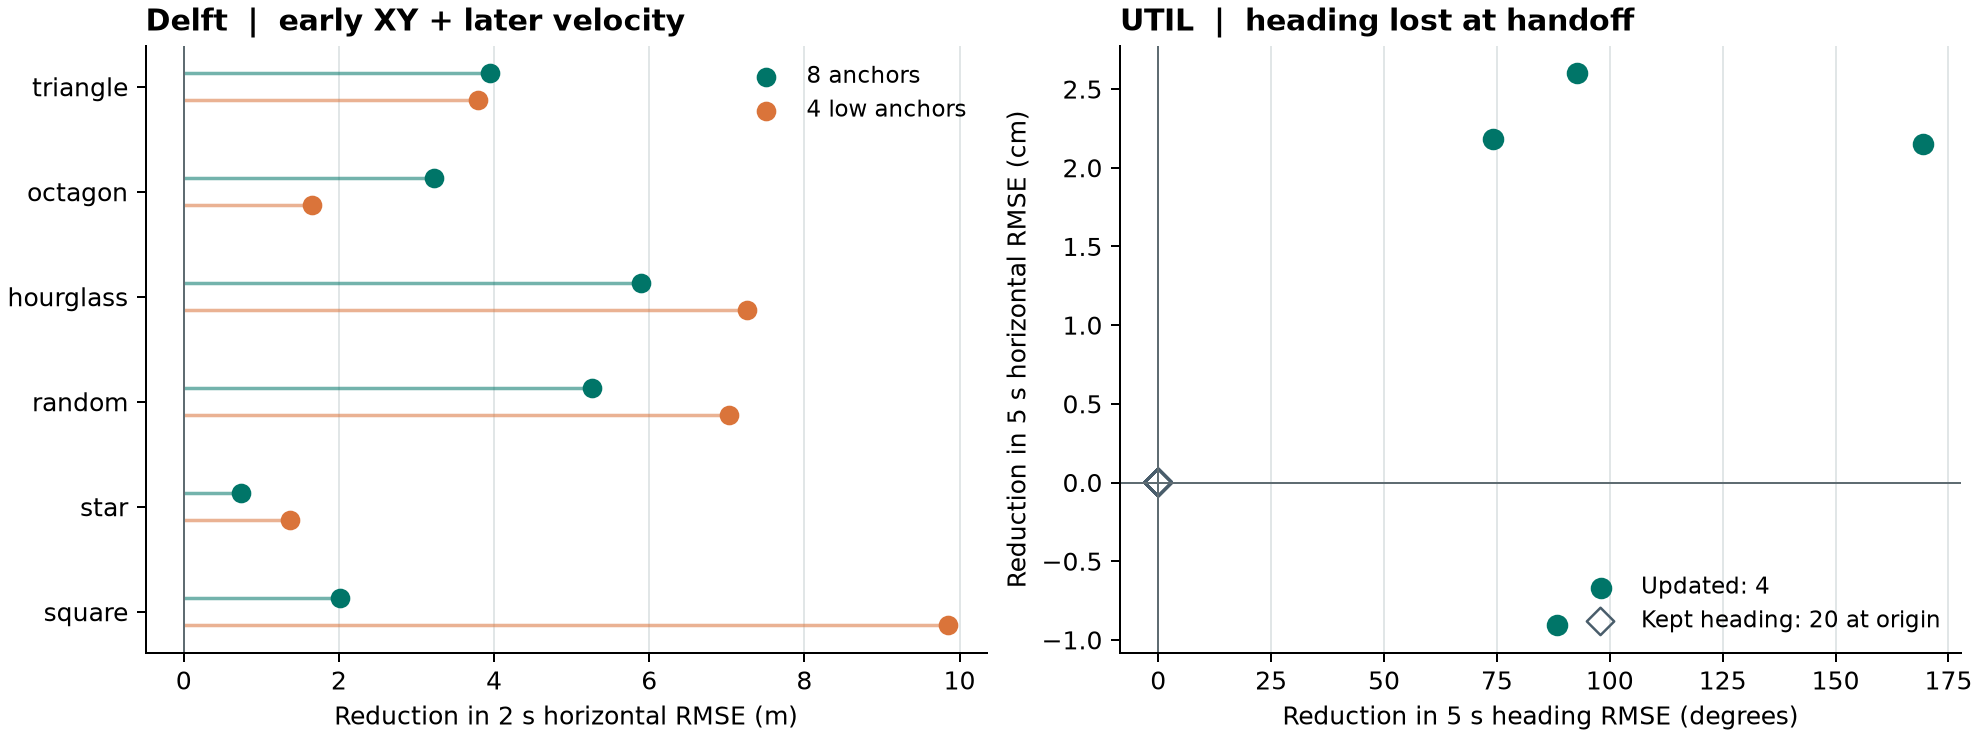
\includegraphics[width=.89\linewidth]{recovery_comparison.png}\\[-1mm]
{\footnotesize\color{muted} 左：Delft 每条录制四角度的配对改善中位数。右：UTIL 交接时受扰；20 个未更新条件重合在原点。}\end{center}

\newpage
\titleblock{02 \quad 真实 TWR 断距}{水平先交接，不能省掉对速度的检查}
Delft 使用六条较晚录制、八锚与最低四锚。每条在第 15 秒给当前估计施加 \(0,+90,-90,180^\circ\) 世界竖轴扰动，物理屏蔽 \([15,25)\unit s\) 的 UWB，得到每布局 24 个配对条件；各策略共享断距前状态与真实 IMU。测距标定来自独立早录。没有可用的评估航向真值，动捕位置仅用于评分与界定有效记录。

\topic{恢复最初两秒，与之后五秒分别评分}
\begin{center}\small
\begin{tabular}{lrrrr}\toprule
 & \multicolumn{2}{c}{25--27 s：XY RMSE / m} & \multicolumn{2}{c}{31--36 s：XY RMSE / m}\\
 & 八锚 & 低位四锚 & 八锚 & 低位四锚\\\midrule
等 2 s，再交接 \(p,v\) &12.370&14.878&0.094&0.145\\
首包恢复普通 InEKF &3.001&3.369&4.153&6.175\\
只早交 XY，之前惯性输出 &1.979&3.476&0.094&0.154\\
只早交 XY，之前普通 InEKF 输出 &0.453&1.701&0.094&0.154\\
早交 XY，再重建 \(p,v\)，之前惯性输出 &1.979&3.347&0.094&0.145\\
早交 XY，再重建 \(p,v\)，之前普通 InEKF 输出 &\textbf{0.448}&\textbf{1.414}&0.094&0.145\\
\bottomrule\end{tabular}\end{center}
表内为逐条件径向 XY RMSE 的中位数。最后一行先输出普通 InEKF，检测通过后切换到预留测量的分支，首次只写 XY；其后，将收到的每锚事务分为两组，用一组跟踪、一组在 27 s 重建 \(p,v\)，保留当时的姿态和偏置。不合并并行后验，不重用预留事务。相比首包普通 InEKF，最初两秒八锚 19/24、四锚 21/24 改善；按每条录制先取配对差中位数，两布局均为 6/6 改善。

低位四锚的未来最坏 XY：只早交 XY 为 \(64.730\unit m\)，分两次交接为 \(1.113\unit m\)，固定等待为 \(0.328\unit m\)。分两次交接显著降低了前两秒的典型误差，未超过固定等待的尾部表现；切换前两布局的最坏瞬时误差仍有 \(42.83/46.51\unit m\)。四锚高度跨度约 0.49 m，并非严格共面。

\topic{独立的航向消融}
另一组固定日程在 27 s 共同重建 \(p,v\)，27--31 s 将每个锚实际收到的事务按奇偶分给在线 InEKF 与旁路证据；31 s 再分叉，只允许姿态动作不同。之后 \([31,36)\) s 的 XY 中位数（米）如下，不能和上表不同分流、不同协方差操作混算。
\begin{center}\small
\begin{tabular}{lrrrr}\toprule
布局 & 保留航向 & 完整姿态 & 强制同候选航向 & 证据通过才更新\\\midrule
八锚     &0.096320&0.095291&0.095146&0.096107\\
低位四锚 &0.148245&0.139875&0.139657&0.148245\\\bottomrule\end{tabular}\end{center}
门控共通过 8/48 次，4 次改善、4 次恶化。没有看到可归因于该门控的稳定 XY 增益。完整姿态求解有 8 次未报告收敛，均保留。八锚和四锚属于同一场地；四个人为角度不是四次独立飞行。

\newpage
\titleblock{03 \quad 真实 TDoA 与初始航向}{改善航向并不等于改善下一段 XY}
\topic{固定准则从绝对距离迁移到距离差}
UTIL trial 1 全部八个预定录制，断距 10--20 s，断距开始时注入 \(0/180^\circ\)。仅换原生 TDoA 观测函数和传感器噪声，水平交接门限沿用 Delft。恢复头两秒，普通 InEKF / 固定等 2 s 再交 \(p,v\) / 提前只交 XY 的中位 RMSE 为 \(\mathbf{16.736/11.741/1.694}\unit m\)；26--31 s 为 \(12.517/0.0531/0.0507\unit m\)。此试验早交分支没有第二次重置。14/16 条件在 0.10 s 内触发，另两例因残差过大等到 3.40 s，全部纳入评分；早窗对普通 InEKF 为 13 胜 3 负。

\topic{保留原速度与重建速度的区别}
另对未用于开发的 trial 4/5 共 16 条录制，在冷启动 / 运动中 / 断距恢复做 \(0,\pm90,180^\circ\) 初始扰动。共同重建 \(p,v\) 后，保留航向 / 完整姿态 / 航向门控的未来 XY 中位数分别为：冷启动 \(0.07372/0.07262/0.07372\unit m\)，运动中 \(0.06759/0.06752/0.06759\unit m\)，断距恢复 \(0.06647/0.06632/0.06647\unit m\)。各窗评到约 45 s；门控 192 个条件全拒。另取相同的 \(0/180^\circ\) 恢复子集：只写 \(p\)、留原速度和航向为 \(0.12856\unit m\)（31/32 完成）；同样只写 \(p\) 再覆完整姿态为 \(0.09168\unit m\)（28/32 完成）；重建 \(p,v\)、留航向为 \(0.06780\unit m\)（32/32 完成）。失例不以截短轨迹充当完整时段。
\topic{刻意让航向在交接当下仍然出错}
为与更早的初始扰动区分，另对 UTIL trial 7 的真实手飞录制在决策瞬间施加 \(0,\pm90,180^\circ\) 估计参考跳变；真实 IMU、无线及物理轨迹不变。四几何交叉两个协议的八个预定槽中只有三槽有录制，采用事先确定的文件名规则；未用其他试次补缺。每条做普通动态窗与断距恢复窗，共 24 个基础条件。各分支共享真实运行至窗末的 \(p,v,b,P\) 并只分叉姿态。
\begin{center}\small\begin{tabular}{llrr}\toprule
场景 & 方法 & 未来 5 s XY 中位数 / m & 航向 RMSE 中位数 / 度\\\midrule
动态 & 保留 / 门控 & 0.121 / 0.116 & 84.87 / 11.61\\
动态 & 强制同一候选 / 完整姿态 & 0.117 / 0.118 & 5.14 / 5.16\\
断距恢复 & 保留 / 门控 & 1.424 / 1.424 & 87.99 / 87.99\\
断距恢复 & 强制同一候选 / 完整姿态 & 1.410 / 1.412 & 14.67 / 11.81\\\bottomrule\end{tabular}\end{center}
仅 4/24 次通过，均在动态段；三次 XY 改善、一次恶化，全部配对的 XY 变化中位数为零。另一试次 8 条录制至多四次重试，32 个条件仅 4 次先拒后收，未来 XY 两胜两负、28 次相同。

\topic{为什么两个指标会分离}
若水平惯性位移为 \(d_h\)，航向误差 \(e\) 单独引起的开环水平位移误差是 \(2\|d_h\|\,|\sin(e/2)|\)。水平机动越弱或后续无线越密，降低航向角误差对闭环 XY 的影响越可能小。反过来，连续相干的错误测距能拟合另一条物理轨迹：留块预测通过也不能证明物理航向正确。

\topic{直接在 Oursland 原滤波器上只加「早交 XY」}
对 trial 4 的四构型、两协议、\(0/180^\circ\) 初始扰动，原推荐先验；在 20 s 恢复时复制完整作者滤波器。各方法之前共用同一轨迹，触发时新分支仅写 XY，之后双方仍运行原作者类。16/16 触发且三窗均完整。原四录制恢复头两秒 XY 中位数为原法/新增交接 \(0.997/1.002\unit m\)，互补四录制 \(0.924/0.925\unit m\)；26--45 s 两组分别为 \(0.11165/0.08683\unit m\)（仅 3/8 对改善）和 \(0.07046/0.07088\unit m\)。因此可辨识的 XY 不意味着覆盖一个本已较准的估计就有净收益。此处初始航向扰动在启动时注入，不是本页开头的断距当下扰动。

\newpage
\titleblock{04 \quad 两个外部基准}{原文、原法回放与共同后端不能混算}
\topic{Oursland 与 Mehrabian：直接运行作者的 InEKF}
RO-MAN 2024 原文摘要报告：初始航向差 \(180^\circ\) 时，InEKF 的航向 RMS 为 \(0.08\unit{rad}\)（4.6°），参考 ESKF 为 \(1.34\unit{rad}\)；图 4 的初角试验排除了构型 3 手飞。这是作者对自己的 ESKF 比较，既不是 XY 数值，也不是我们的实测改善。独立运行未修改的作者类；在一个保留作者原始真值初始化和原生时序的 45 s 健康检查里，其 XY 为 \(0.0468\unit m\)、航向为 3.74°。无真值初始化比较另行配对，不能把此检查当成相同输入先验。
四条预定 UTIL 录制覆盖四种基站构型与两种协议，各取 \(0/180^\circ\)；双方相同的传感器初始化、作者推荐初始 \(P\)、原始无线方差和原生事件队列。作者类不修改，各方法每场景 8/8 完成。表中自固定交接时刻评至约 45 s，XY 单位米，航向单位度。
\begin{center}\small\begin{tabular}{lrrr}\toprule
方法（XY / 航向 RMSE 中位数） & 弱冷启动 & 运动中 & 断距恢复\\\midrule
Oursland 原类连续递推 & \textbf{0.0762 / 6.72} & \textbf{0.0782 / 6.66} & 0.1118 / \textbf{5.93}\\
本次 \(p,v\) 交接、留航向 & 0.0843 / 60.76 & 0.0825 / 43.67 & \textbf{0.0872} / 40.15\\
本次 \(p,v\) 加完整姿态交接 & 0.0781 / 32.97 & 0.0802 / 47.24 & 0.0892 / 65.42\\\bottomrule
\end{tabular}\end{center}
航向门控 24 个条件全拒，结果等于留航向。后者恢复段 XY 虽有较低中位数，却只赢 4/8 个配对，且航向明显落后原作者；弱冷启动和运动中，作者连 XY 也更好。这里比较的是整套方法。

\topic{Theodosis 等：单锚二次量测观测器}
arXiv:2006.02688v2 第 6 节假设已知世界系加速度 \(u\)，量测 \(y=\frac12\|p\|^2\)。源法无姿态状态；以 \(q_0=p^\top p/2,\ q_1=p^\top v,\ q_2=v^\top v\) 扩充运动学，得
\(\dot q_0=q_1,\ \dot q_1=q_2+p^\top u,\ \dot q_2=2v^\top u\)。
按实际九维状态和标量量测修正原文印刷的矩阵维度，取未指定初估为零；在其无噪富激励仿真中，20 s 位置/速度误差复现值为 \(0.0957\unit m/0.0118\unit{m/s}\)。

对真实多锚 TWR 的显式扩展为
\[
 \tfrac12(r_j^2-\sigma_j^2-\|a_j\|^2)=q_0-a_j^\top p+\epsilon_j,\qquad
 \operatorname{var}(\epsilon_j\mid p)=\|p-a_j\|^2\sigma_j^2+\tfrac12\sigma_j^4
\]
（后一式按零均值高斯距离噪声）。用共同 IMU 推出的世界加速度，不喂动捕姿态。下表在同一 25--27 s 前端窗口后使用相同的保留航向 InEKF 后端；射频事件、物理协方差操作与评分时钟均一致。
\begin{center}\small\begin{tabular}{llrrr}\toprule
布局 & 位置前端 & 交接瞬间 XY / m & 31--36 s XY / m & 同期 Z / m\\\midrule
八锚 & 原生距离窗 &0.192&0.09632&0.270\\
     & 二次观测器多锚扩展 &\textbf{0.085}&0.09632&0.270\\
低位四锚 & 原生距离窗 &0.182&\textbf{0.14825}&0.983\\
         & 二次观测器多锚扩展 &\textbf{0.169}&0.18992&1.006\\\bottomrule\end{tabular}\end{center}
低位四锚的后续差异集中在个别录制，多数配对差很小。原生单锚另按相同一个锚和世界输入，对照六维距离 EKF：31--36 s 的 XY 中位数为 \(28.139/9.866\unit m\)。这既不是原文报道的实飞误差，也不能算作我们完整多锚系统优于单锚理论的倍数。
\vfill{\footnotesize\color{muted} 外部来源：J. Oursland \& M. Mehrabian, IEEE RO-MAN 2024, DOI 10.1109/RO-MAN60168.2024.10731434；D. Theodosis, S. Berkane \& D. V. Dimarogonas, arXiv:2006.02688v2，2020。逐例数据、代码和全部失例见项目 experiments/split\_handoff。}
\end{document}
